\section{Objets DICOM}

\frame
{
 	\frametitle{Information Object Definition}
  	L'IOD d\'etermine, pour un IO sp\'ecifique, quelles sont les valeurs qu'on doit ou peut trouver dans l'objet.
  	\begin{description}
    		\item<2->[Normalized IOD]~\\
			Repr\'esente une entit\'e unique du monde r\'eel (patient, visite, examen, r\'esultat, interpr\'etation,\ldots).
			Rarement appliqu\'e en pratique : cause complexit\'e et perte de performance.
    		\item<3->[Composite IOD]~\\
			Repr\'esente certains d\'etails de plusieurs objets du monde r\'eel et les relations entre ces objets (nom du patient, date de l'examen,\ldots)
		\item<4->[Attributes]~\\
			Les attributs d'un IOD d\'ecrivent les propri\'et\'es d'un \'el\'ement (instance d'un objet) du monde r\'eel.
  	\end{description}
}

\frame
{
 	\frametitle{IOD composite}
 	\begin{itemize}
		\item<1-> IOD compos\'es d'\emph{Information Entities} ou \emph{IE}.
   		\item<2-> Une IE comporte un ou plusieurs \emph{Modules} (= ensemble de valeurs li\'ees).
		\begin{description}
			\item<3->[Mandatory] Module obligatoire.
			\item<4->[Conditional] Module conditionnel (obligatoire selon certaines conditions).
			\item<5->[User Option] Module optionnel.
		\end{description}
   		\item<6-> Les modules sont compos\'es d'\emph{Attributs} (= valeurs).
		\begin{description}
			\item<7->[1] Obligatoire.
			\item<8->[2] Obligatoire - peut \^etre vide.
			\item<9->[3] Optionnel.
			\item<10->[<1/2>C] Conditionnel.
		\end{description}
 	\end{itemize}

	\begin{alertblock}{En pratique}<11->
		Un objet DICOM est presque toujours une instance d'un IOD composite.
	\end{alertblock}
}

\frame
{
	\frametitle{Exemple d'IOD : image CR}
	
	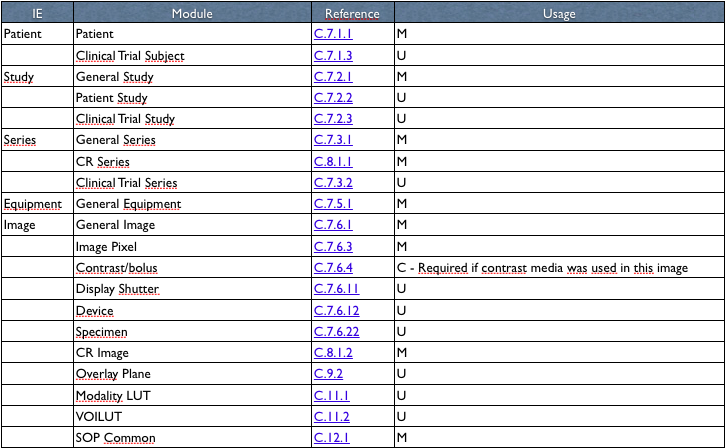
\includegraphics[width=\linewidth]{./figures/IOD-exemple.png}
}

\frame
{
	\frametitle{Information Object Defintion (IOD)}
	
	\begin{center}
		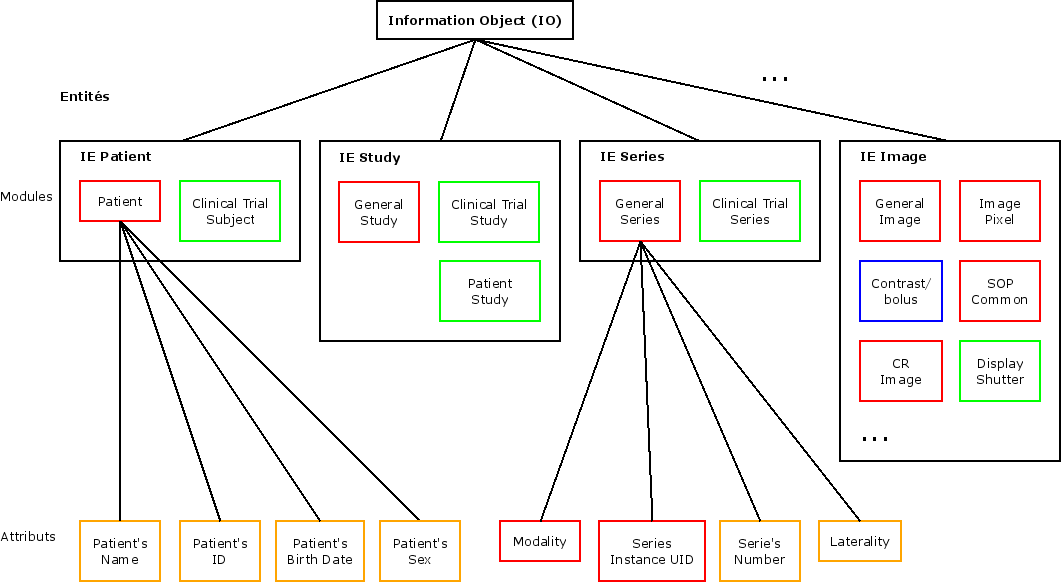
\includegraphics[width=\linewidth]{./figures/IO-definition.png}
	\end{center}
}

\frame
{
	\frametitle{Objet}
	\begin{itemize}
		\item<1-> Terminologie : objet = Data Set (= ensemble de donn\'ees).
		\item<2-> Un Data Set est compos\'e de Data Elements.
		\item<3-> Chaque Data Element instancie un attribut de l'IOD.
		\item<4-> Data Element
		\begin{itemize}
			\item<5-> �tiquette d'identification (\emph{Tag}) contenant deux num\'eros.
			\item<6-> Type (\emph{VR} = \emph{Value Representation}).
			\item<7-> Taille de la valeur.
			\item<8-> Valeur.
		\end{itemize}
	\end{itemize}
}

\frame
{
	\frametitle{Objet}
	
	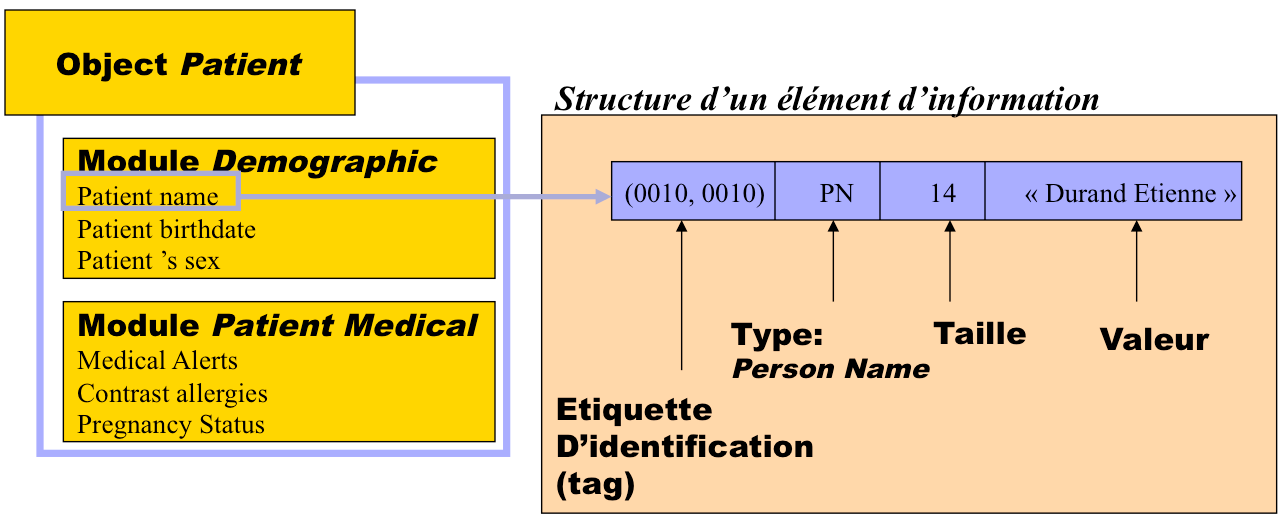
\includegraphics[width=\linewidth]{./figures/objet-dicom.png}
}

\frame
{
	\frametitle{Exemple d'objet : Examen (\emph{Study})}
	
	\begin{center}
		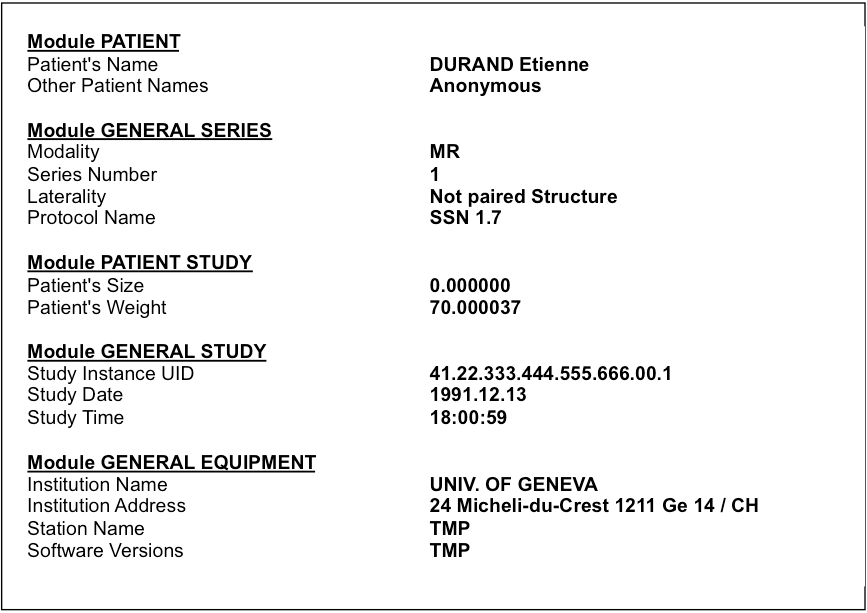
\includegraphics[width=.9\linewidth]{./figures/examen.png}
	\end{center}
}

\frame
{
	\frametitle{Exemple d'objet : Image IRM}
	
	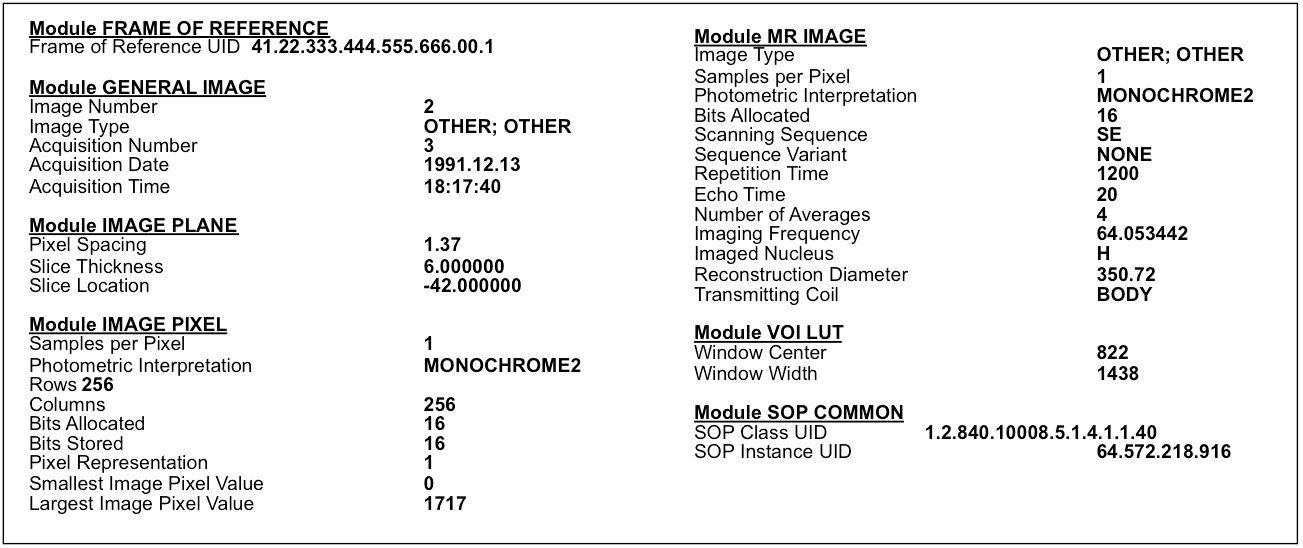
\includegraphics[width=\linewidth]{./figures/irm.png}
}

\frame
{
	\frametitle{Fichier DICOM}
	
	\begin{itemize}
		\item Encapsuler l'ensemble des objets dans un fichier.
		\begin{itemize}
			\item<2-> Ent\^ete : pr\'e-ent\^ete et objets.
			\item<3-> Image : donn\'ees brutes de l'image.
		\end{itemize}
		\item<4-> Les d\'etails au prochain cours.
	\end{itemize}
}

